\section{Agentes Inteligentes}

En el ámbito de la inteligencia artificial, un agente inteligente es un sistema computacional 
diseñado para interactuar con su entorno de manera autónoma. Este sistema utiliza sensores 
para recibir información del entorno y actuadores para realizar acciones en respuesta a esa 
información. Su objetivo es percibir su entorno, procesar esa información de manera interna y 
tomar decisiones basadas en un conjunto de reglas o algoritmos predefinidos. Es como si fuera 
el cerebro y el cuerpo de una máquina, capaz de observar, pensar y actuar de manera inteligente 
para lograr sus objetivos en el mundo real.\\


En términos simples, el ejemplo de un carro autónomo como un agente inteligente es que percibe su
entorno con \textit{sensores} instalados que le permiten recopilar información sobre la carretera,
otros autos y peatones. Luego, procesa toda esa información para tomar decisiones lógicas y 
razonables sobre cómo manejar \textit{actuadores}, como cambiar de carril de manera segura, 
frenar para evitar colisiones o girar en una intersección basándose en lo que ha observado y en 
las reglas de tránsito. 

\begin{center}
    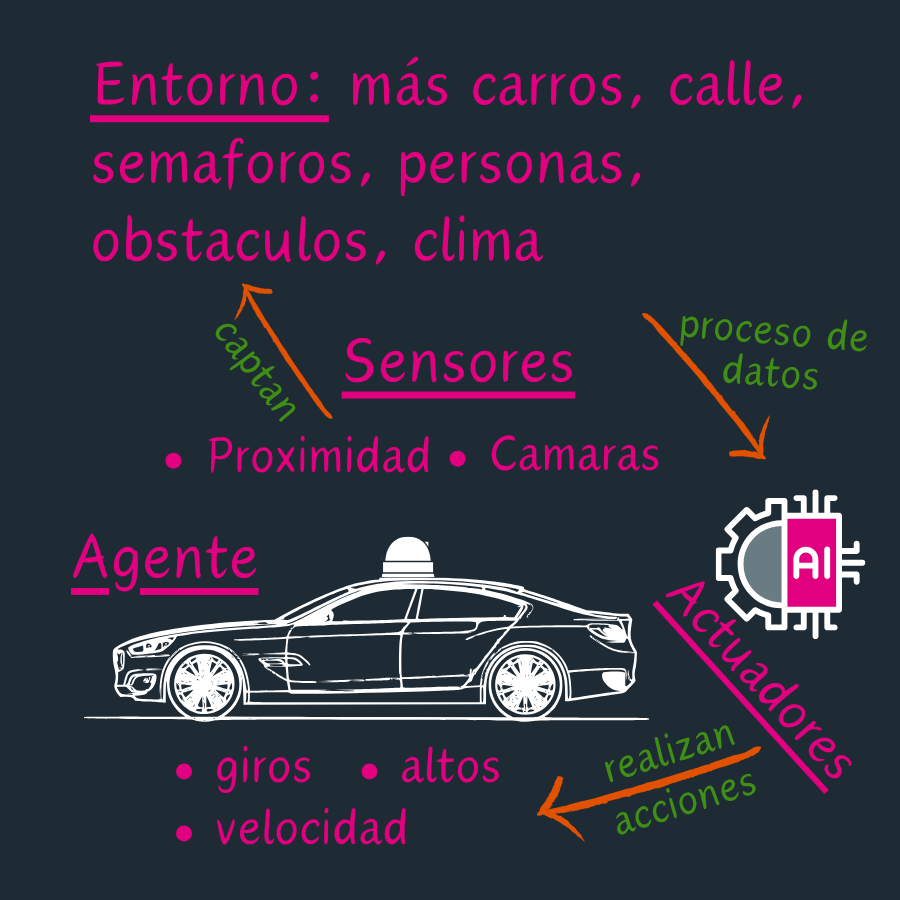
\includegraphics[scale = .6]{assets/imagenes/agenInte.png}
\end{center}

% -------------------------------------------------------------------------------------/
% ------------------------------------------------------------------------------------/
% -----------------------------------------------------------------------------------/
\subsection*{Propiedades}
% -------------------------------------------------------------------------------------/
% ------------------------------------------------------------------------------------/
% -----------------------------------------------------------------------------------/

\begin{enumerate}
    \item Adaptabilidad: Esto significa que los agentes pueden aprender y cambiar su comportamiento 
    según lo que descubren. Es como aprender de tus errores y hacer las cosas de 
    manera diferente la próxima vez.

    \item Reactividad: Los agentes actúan en respuesta a lo que está sucediendo a su alrededor. 
    Por ejemplo, si ven un obstáculo en el camino, cambian de dirección para evitarlo.
    
    \item Racionalidad: Significa hacer siempre lo correcto según lo que ven y escuchan. Es como 
    tomar decisiones inteligentes basadas en la información disponible.
    
    \item Pro-actividad: Es cuando los agentes pueden decidir por sí mismos qué hacer, incluso si 
    el entorno cambia. Es como tener un plan y seguirlo aunque las cosas cambien.
    
    \item Toma de decisiones: Los agentes usan su inteligencia artificial para tomar decisiones 
    inteligentes. Pueden seguir reglas o aprender de la experiencia para hacerlo mejor con el tiempo.
    
    \item Actuación: Después de decidir qué hacer, los agentes actúan en su entorno a través de 
    sus manos mágicas (actuadores). Esto puede afectar lo que está sucediendo a su alrededor y 
    ayudarlos a alcanzar sus objetivos.
    
    \item Continuidad Temporal: Los agentes siguen funcionando sin parar, como una película que 
    nunca termina. Siempre están listos para actuar y hacer lo que sea necesario.
    
    \item Autonomía: Significa que los agentes pueden tomar decisiones por sí mismos y adaptarse 
    a los cambios en su entorno.
    
    \item Aprendizaje: Algunos agentes pueden aprender de sus errores y experiencias pasadas para 
    mejorar en el futuro. Es como aprender de tus errores y hacerlo mejor la próxima vez.
    
    \item Sociabilidad: Algunos agentes pueden comunicarse con otros agentes o entidades, como 
    hablar con amigos en las redes sociales.
    
    \item Movilidad: Algunos agentes pueden moverse a través de una red de computadoras, como 
    navegar por internet en tu teléfono.
    
    \item Veracidad: Los agentes siempre dicen la verdad y no engañan a propósito.
    
    \item Cooperatividad: Los agentes están dispuestos a ayudar si eso no entra en conflicto con 
    sus propios objetivos. Es como trabajar juntos para lograr algo grande.    
\end{enumerate}


% -------------------------------------------------------------------------------------/
% ------------------------------------------------------------------------------------/
% -----------------------------------------------------------------------------------/
\subsection*{Tipos de agentes}
% -------------------------------------------------------------------------------------/
% ------------------------------------------------------------------------------------/
% -----------------------------------------------------------------------------------/

\begin{myitemize}
    \item Agente de reactivo simple
    \begin{myitemize}
        \item Definición: Este tipo de agente toma decisiones basadas únicamente en la percepción actual de su entorno, sin tener en cuenta información pasada ni futuro. Actúa de manera inmediata y directa en respuesta a estímulos.
        \item Utilidad: Son útiles en entornos simples y con reglas claras, donde las respuestas pueden ser predefinidas.
        \item Importancia y características: Son rápidos y eficientes en situaciones específicas, pero pueden no ser adecuados para entornos dinámicos o complejos.
        \item Ejemplo: Un robot aspirador que se mueve hacia adelante si no hay obstáculos y se detiene si detecta uno.
        \item Cumple con: Reactividad, actuación.
        \item Limitaciones: Puede ser limitado en entornos complejos donde se requiere planificación a largo plazo o consideración de múltiples factores simultáneamente.
    \end{myitemize}
    
    \item Agente reactivo basado en modelo    
    \begin{myitemize}
        \item Definición: Este tipo de agente también se basa en la percepción actual del entorno, pero incorpora un modelo interno que le permite anticipar el resultado de sus acciones.
        \item Utilidad: Son útiles en entornos dinámicos donde se pueden anticipar cambios y adaptarse en consecuencia.
        \item Importancia y características: Tienen la capacidad de tomar decisiones más informadas y planificadas en comparación con los agentes de reactivo simple.
        \item Ejemplo: Un vehículo autónomo que utiliza modelos de predicción del tráfico para planificar sus movimientos.
        \item Cumple con: Reactividad, adaptabilidad, toma de decisiones.
        \item Limitaciones: La precisión del modelo interno puede verse afectada por cambios inesperados en el entorno o por la falta de datos históricos relevantes.                
    \end{myitemize}

    \item Agente basado en metas    
    \begin{myitemize}
        \item Definición: Estos agentes tienen objetivos definidos y trabajan para alcanzarlos, tomando decisiones que maximicen la probabilidad de lograr esas metas.
        \item Utilidad: Son útiles en entornos donde se pueden definir objetivos claros y se requiere planificación a largo plazo.
        \item Importancia y características: Son capaces de tomar decisiones orientadas hacia el logro de metas específicas, incluso en entornos complejos y cambiantes.
        \item Ejemplo: Un asistente virtual que tiene como objetivo ayudar al usuario a completar tareas diarias, como recordar citas o hacer listas de compras.
        \item Cumple con: Pro-actividad, toma de decisiones, autonomía.
        \item Limitaciones: La precisión del modelo interno puede verse afectada por cambios inesperados en el entorno o por la falta de datos históricos relevantes.
    \end{myitemize}
    
    \item Agente basado en utilidad    
    \begin{myitemize}
        \item Definición: Este tipo de agente evalúa las posibles acciones en función de su utilidad o beneficio esperado y elige la acción que maximice esa utilidad.
        \item Utilidad: Son útiles en entornos donde hay múltiples acciones posibles y se debe elegir la mejor opción en función de un criterio de valor.
        \item Importancia y características: Toman decisiones racionales y óptimas en situaciones donde hay múltiples objetivos o preferencias a considerar.
        \item Ejemplo: Un sistema de recomendación en línea que sugiere películas basadas en las preferencias pasadas del usuario y las calificaciones de otros usuarios.
        \item Cumple con: Racionalidad, toma de decisiones.
        \item Limitaciones: La asignación de valores de utilidad puede ser subjetiva y estar sujeta a cambios en las preferencias del usuario, lo que puede afectar la efectividad del agente.
    \end{myitemize}

    \item Agente que aprende
    \begin{myitemize}
        \item Definición: Estos agentes tienen la capacidad de mejorar su rendimiento con el tiempo a través del aprendizaje, ya sea mediante la adaptación de reglas existentes o la adquisición de nuevas.
        \item Utilidad: Son útiles en entornos donde los datos son cambiantes o incompletos, y se requiere flexibilidad para adaptarse.
        \item Importancia y características: Son capaces de ajustar su comportamiento en función de la experiencia pasada, lo que les permite mejorar su desempeño en diferentes situaciones.
        \item Ejemplo: Un algoritmo de recomendación de música que aprende los gustos musicales del usuario a medida que interactúa con la plataforma.
        \item Cumple con: Adaptabilidad, aprendizaje.
        \item Limitaciones: La dependencia de datos pasados puede llevar a decisiones sesgadas o a la dificultad de adaptarse a cambios repentinos en el entorno.
    \end{myitemize}
    
    \item Agente de consulta
    \begin{myitemize}
        \item Definición: Estos agentes recopilan información de diversas fuentes y la presentan al usuario en forma de respuestas o recomendaciones.
        \item Utilidad: Son útiles cuando se necesita acceder y procesar grandes cantidades de datos para proporcionar información útil al usuario.
        \item Importancia y características: Son capaces de filtrar y presentar información relevante de manera organizada, lo que facilita la toma de decisiones por parte del usuario.
        \item Ejemplo: Un motor de búsqueda en internet que recopila y presenta resultados relevantes a partir de consultas de los usuarios.
        \item Cumple con: Percepción del entorno, toma de decisiones, actuación.
        \item Limitaciones: La calidad de las respuestas proporcionadas puede verse afectada por la disponibilidad y precisión de la información en las fuentes consultadas, así como por la capacidad del agente para procesarla de manera efectiva.
    \end{myitemize}
\end{myitemize}

% -------------------------------------------------------------------------------------/
% ------------------------------------------------------------------------------------/
% -----------------------------------------------------------------------------------/
\subsection*{Tipos de entornos}
% -------------------------------------------------------------------------------------/
% ------------------------------------------------------------------------------------/
% -----------------------------------------------------------------------------------/

Los entornos en los que operan los agentes inteligentes son fundamentales para comprender su
funcionamiento y desempeño. Un entorno proporciona el contexto en el cual un agente toma
decisiones y realiza acciones para alcanzar sus objetivos.\\ 

El diseño de agentes inteligentes se basa en comprender los entornos en los que operan, ya 
que estos proporcionan el contexto para que los agentes tomen decisiones y ejecuten 
acciones para lograr sus objetivos. 

\noindent \textcolor{Contraste4}{Elementos de los Entornos de Trabajo}\\

\begin{myitemize}
    \item Observaciones: Son la información que el agente recibe del entorno, ya sea completa o parcial. Esto depende de si el agente tiene acceso a toda la información relevante o solo a una parte.
    \item Acciones: Representan las decisiones que el agente puede tomar para influir en su entorno. Pueden ser discretas o continuas, y la elección de acciones afecta el estado del ambiente.
    \item Recompensas: Son señales de retroalimentación que el agente recibe del ambiente después de realizar una acción. Informan al agente sobre la calidad de su acción en términos de sus objetivos.
    \item Estados: Representan la situación actual del ambiente. Pueden ser completamente observables o parcialmente observables, y el agente toma decisiones basadas en su percepción del estado actual.
    \item Dinámica del Ambiente: Describe cómo evoluciona el ambiente con el tiempo en respuesta a las acciones del agente y posiblemente a eventos externos. Puede ser estocástica, lo que significa que hay elementos de incertidumbre.
    \item Espacio de Acciones y Observaciones: Constituye el conjunto de todas las acciones posibles que el agente puede realizar y el conjunto de todas las observaciones posibles que puede recibir.
\end{myitemize}


\noindent \textcolor{Contraste4}{Propiedades Adicionales de los Entornos de Trabajo}\\

\begin{myitemize}
    \item Totalmente observable vs. parcialmente observable: Depende de si los sensores del agente proporcionan acceso al estado completo del entorno en cada momento.
    \item DeteEpisódico vs. secuencial: En entornos episódicos, la experiencia del agente se divide en episodios atómicos, mientras que en entornos secuenciales, la decisión presente puede afectar a decisiones futuras.
    \item Estático vs. dinámico: Determina si el ambiente puede cambiar mientras el agente está deliberando.
    \item Discreto vs. continuo: Se aplica al estado del medio, la forma en la que se maneja el tiempo y las percepciones y acciones del agente.
    \item Agente individual vs. multiagente: Se refiere a si el agente interactúa con otros agentes en su entorno y cómo estas interacciones afectan su comportamiento.
\end{myitemize}


\noindent \textcolor{Contraste4}{Evaluación del agente}\\

\begin{enumerate}
    \item Medición de Desempeño:
    \begin{myitemize}
        \item Métricas Específicas: Define métricas específicas relevantes para la tarea. Por ejemplo, si el agente está
        diseñado para jugar juegos, se podrían usar métricas como la tasa de victorias, la puntuación media o la
        eficiencia en el uso de recursos.

        \item Precisión: En tareas como clasificación o reconocimiento, se puede evaluar la precisión del agente en la
        toma de decisiones correctas.        
    \end{myitemize}
    \item Comparación con Humanos
    \begin{myitemize}
        \item Benchmarking: Compara el rendimiento del agente con el de humanos. Esto puede incluir la comparación
        de la tasa de error, el tiempo de ejecución o cualquier otra métrica relevante.

        \item Crowdsourcing: Utiliza la opinión de un grupo de personas para evaluar la calidad de las decisiones o
        acciones del agente.        
    \end{myitemize}
    \item Validación Cruzada
    \begin{myitemize}
        \item Divide los datos en conjuntos de entrenamiento y prueba para evaluar el rendimiento del agente en datos no
        vistos. La validación cruzada puede ayudar a identificar problemas de sobreajuste o subajuste.
    \end{myitemize}

    \item Aprendizaje en Línea
    \begin{myitemize}
        \item Evalúa el rendimiento del agente a medida que aprende de nuevas instancias. Esto es
        especialmente relevante para agentes que se entrenan continuamente.
    \end{myitemize}


    \item Simulaciones y Entornos de Prueba
    \begin{myitemize}
        \item Utiliza simulaciones o entornos específicos para evaluar el desempeño del agente. Esto es
        común en entornos de robótica o simulaciones virtuales.
    \end{myitemize}


    \item Eficiencia y Recursos
    \begin{myitemize}
        \item Evalúa la eficiencia del agente en términos de tiempo de cómputo, consumo de recursos y
        otros aspectos relacionados con la eficiencia.
    \end{myitemize}


    \item Generalización
    \begin{myitemize}
        \item Evalúa la capacidad del agente para generalizar su aprendizaje a nuevas situaciones o datos
        no vistos.
    \end{myitemize}

    \item Análisis de Fallos
    \begin{myitemize}
        \item Examina los casos en los que el agente falla y analiza las razones detrás de esos fallos. Esto
        puede ayudar a mejorar el agente identificando debilidades específicas.
    \end{myitemize}
\end{enumerate}